\documentclass[12pt]{report}
\usepackage[utf8]{inputenc}
\usepackage{geometry}
\geometry{a4paper, margin=1in}
\usepackage{hyperref}
\usepackage{graphicx}
\usepackage{amsmath}
\usepackage{booktabs}
\usepackage{float}
\usepackage{setspace}
\usepackage{listings}
\usepackage{xcolor}

% Code snippet styling
\definecolor{codegreen}{rgb}{0,0.6,0}
\definecolor{codegray}{rgb}{0.5,0.5,0.5}
\definecolor{codepurple}{rgb}{0.58,0,0.82}
\definecolor{backcolour}{rgb}{0.95,0.95,0.92}

\lstdefinestyle{mystyle}{
    backgroundcolor=\color{backcolour},   
    commentstyle=\color{codegreen},
    keywordstyle=\color{magenta},
    numberstyle=\tiny\color{codegray},
    stringstyle=\color{codepurple},
    basicstyle=\ttfamily\footnotesize,
    breakatwhitespace=false,         
    breaklines=true,                 
    captionpos=b,                    
    keepspaces=true,                 
    numbers=left,                    
    numbersep=5pt,                  
    showspaces=false,                
    showstringspaces=false,
    showtabs=false,                  
    tabsize=2
}
\lstset{style=mystyle}

\begin{document}

% --- TITLE PAGE ---
\begin{titlepage}
    \centering
    \vspace*{2cm}
    
    \Huge
    \textbf{Predictive Analytics in Emerging Markets}
    
    \vspace{0.5cm}
    \LARGE
    End-to-End Machine Learning for Second-Hand Car Prices in Morocco
    
    \vspace{2cm}
    
    \large
    \textbf{Prepared by Group 1:} \\
    \vspace{0.2cm}
    \normalsize
    1. Amine A. \\
    2. [Group Member 2] \\
    3. [Group Member 3] \\
    4. [Group Member 4] \\
    5. [Group Member 5] \\
    6. [Group Member 6] \\
    
    \vspace{2cm}
    
    \large
    \textbf{Supervised by:} \\
    Professor [Professor's Name]
    
    \vfill
    
    \large
    \textbf{University / Institution Name} \\
    \vspace{0.2cm}
    June 2026
\end{titlepage}

\onehalfspacing
\tableofcontents
\newpage

% --- CHAPTER 1 ---
\chapter{Web Scraping and Data Collection}

\section{The Evolution of the Scraper}
To mathematically evaluate the second-hand car market in Morocco, we needed real-world data. We initially built a simple Python scraper using \texttt{BeautifulSoup} and \texttt{Requests} to extract listings from \texttt{moteur.ma}. 

Our first iteration parsed merely 10 to 50 pages. However, to deploy a highly robust Machine Learning model, we required volume. We decided to drastically expand the pagination parameter. We initially considered scraping 1,200 pages, but to avoid hardware overheating and server blocks ("burning the laptop"), we strategically settled on \textbf{500 pages}. This optimal limit yielded over \textbf{15,000 distinct car listings}.

\section{Scraping Methodology}
Below is a core snippet demonstrating how we bypassed constraints and parsed the HTML Document Object Model (DOM) to extract features like Price, Year, and Mileage:

\begin{lstlisting}[language=Python, caption=Core Scraper Logic]
import requests
from bs4 import BeautifulSoup
import pandas as pd

data = []
for page in range(1, 501): # Capped at 500 pages
    url = f"https://www.moteur.ma/fr/voiture/achat-voiture-occasion/recherche/?page={page}"
    response = requests.get(url)
    soup = BeautifulSoup(response.text, 'html.parser')
    
    for car in soup.find_all('div', class_='row-item'):
        title = car.find('h3').text.strip()
        price = car.find('div', class_='price').text.strip()
        data.append({'Title': title, 'Price': price})
\end{lstlisting}

\newpage

% --- CHAPTER 2 ---
\chapter{Exploratory Data Analysis (EDA)}

Before building any mathematical models, we generated descriptive statistics and visual plots to understand how Moroccan buyers value cars.

\section{Price Distribution}
The majority of the Moroccan car market operates heavily within the budget constraint of under 300,000 MAD. However, extreme outliers exist, stretching up to 1,500,000 MAD for luxury vehicles (e.g., Range Rover, Mercedes-Benz G-Class).

\begin{figure}[H]
    \centering
    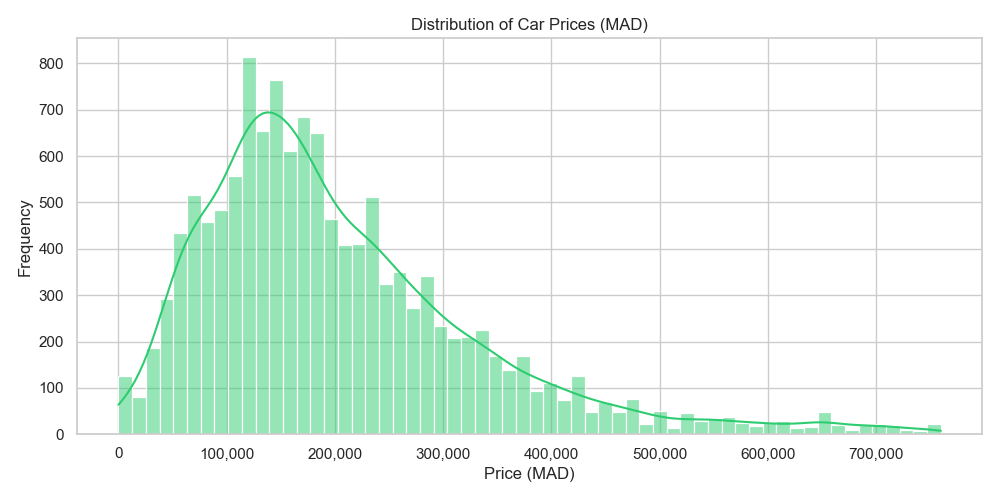
\includegraphics[width=0.8\textwidth]{images/StepB_1_Price_Distribution.png}
    \caption{Distribution of Car Prices (MAD)}
\end{figure}

\section{The Depreciation Curve (Mileage)}
Our scripts visualized the explicit relationship between a car's odometer and its market value. The devaluation curve is steepest between $0$ and $150,000$ km. After the $150,000$ km threshold, the depreciation rate flattens, indicating that older vehicles eventually hit a mathematical "utility floor" where mileage ceases to destroy value.

\begin{figure}[H]
    \centering
    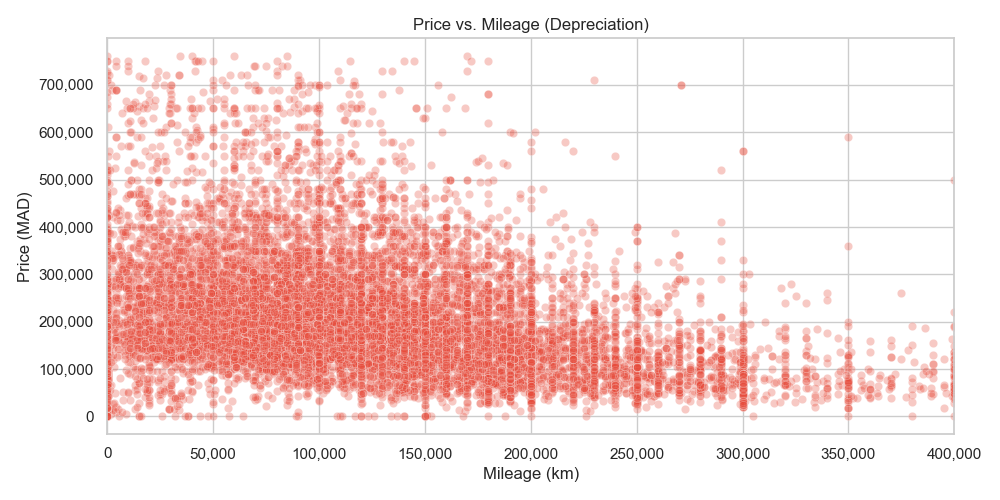
\includegraphics[width=0.8\textwidth]{images/StepB_2_Price_vs_Mileage.png}
    \caption{Scatter Plot: Price Depreciation vs. Mileage}
\end{figure}

\section{Brand and Categorical Dominance}
We discovered that Automatic transmissions command a heavy premium over Manual configurations. Additionally, Diesel is the absolute dominant fuel type in Morocco, though Hybrid vehicles show the highest initial retention value.

\begin{figure}[H]
    \centering
    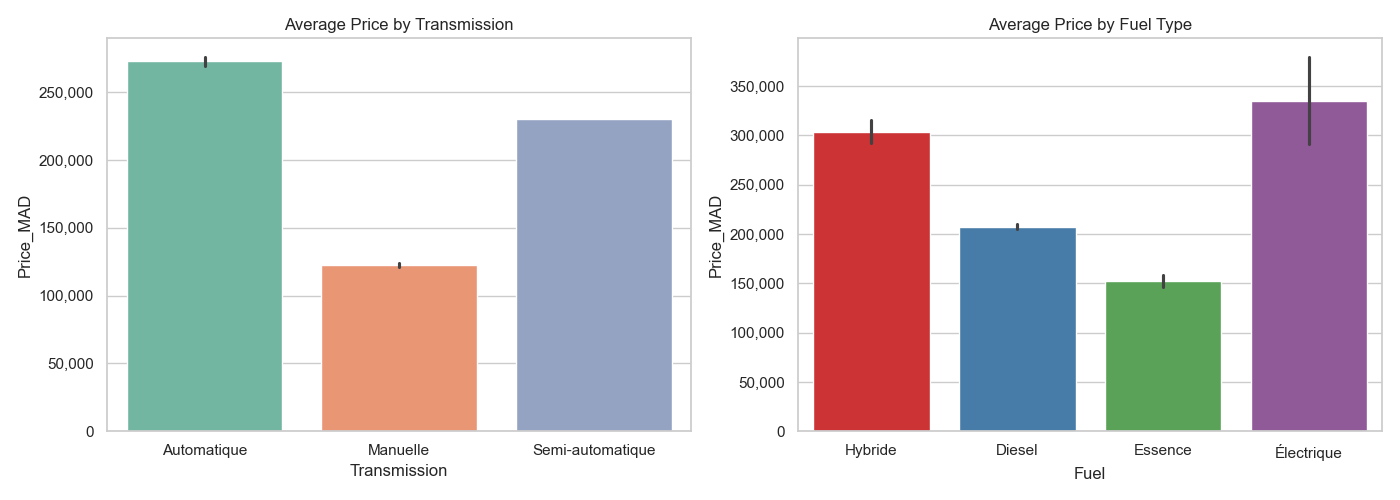
\includegraphics[width=0.8\textwidth]{images/StepB_4_Price_vs_Categoricals.png}
    \caption{Boxplots of Price variations across Transmission and Fuel Types}
\end{figure}

\newpage

% --- CHAPTER 3 ---
\chapter{Machine Learning Iterations (V1 - V5)}

The true engineering challenge of this project lay in optimizing the predictive algorithm. Over 5 iterations, we dropped our Error Margin from 52,000 MAD down to 16,000 MAD.

\section{Version 1: The Generic Baseline}
\textbf{The Goal:} Establish a baseline mathematical prediction using basic features. \\
\textbf{What we did:} We used One-Hot Encoding to convert categories into booleans and applied a standard Random Forest Regressor. However, we only extracted the parent \texttt{Brand} from the title (e.g., "Mercedes-Benz"). \\
\textbf{The Result:} The model produced a devastating Mean Absolute Error (MAE) of \textbf{52,000 MAD}. It mathematically failed because it could not distinguish between a 300,000 MAD Mercedes A-Class and a 1,500,000 MAD Mercedes G-Class. 

\section{Version 2: Sub-Feature Extraction}
\textbf{The Goal:} Fix the 52k error by introducing model specificity. \\
\textbf{What we did:} We applied complex string manipulation to extract the specific \texttt{CarModel} from the string (e.g., isolating "Classe CLA"). We injected the top 100 Car Models into the matrix.
\begin{lstlisting}[language=Python, caption=Extracting the exact Car Model]
df['Brand'] = df['Title'].apply(lambda x: str(x).split()[0].title())
df['CarModel'] = df['Title'].apply(lambda x: " ".join(str(x).split()[1:]).title())
\end{lstlisting}
\textbf{The Result:} Accuracy jumped to \textbf{70.0\%}, shrinking the error down to \textbf{39,000 MAD}.

\section{Version 3: Target Encoding}
\textbf{The Goal:} Remove the inefficient Boolean matrix. \\
\textbf{What we did:} The boolean "True/False" approach treated locations like "Casablanca" and "El Jadida" equally, failing to acknowledge that major northern cities command higher market baselines. We ripped out One-Hot Encoding and deployed \textbf{Target Encoding}, which mathematically replaces a city name with the \textit{average price of all cars in that city}.
\textbf{The Result:} Dimensionality dropped from 138 columns down to 8. Accuracy surged to \textbf{76.6\%}, and the error dropped to \textbf{35,000 MAD}.

\section{Version 4: Economy vs. Luxury Split}
\textbf{The Goal:} Protect budget car evaluations from millionaire outliers. \\
\textbf{What we did:} We noticed the average car was 177,000 MAD, yet 35,000 MAD was a 20\% error margin. The error was being skewed by the AI trying to predict 1.5 million MAD Range Rovers. We isolated the dataset, training a model exclusively on "Economy" cars ($\le$ 300,000 MAD). \\
\textbf{The Result:} Accuracy exploded to \textbf{87.3\%}, dropping the error margin for average Moroccan cars down to \textbf{16,390 MAD}.

\section{Version 5 (Final): The Hierarchical AI Router}
\textbf{The Goal:} Build a single, unified pipeline capable of predicting \textit{any} car automatically. \\
\textbf{What we did:} Since users do not know if their car is Economy or Luxury until they see the price, we built a \textbf{3-Stage Hierarchical Model}. Furthermore, we combined Brand and Model into a \textit{Feature Cross} to create unique identities (e.g., "Mercedes-Benz Classe CLA").

\begin{enumerate}
    \item \textbf{Stage 1 (Classifier):} A Random Forest Classification network that predicts if a car belongs to the Economy or Luxury tier. (Achieved \textbf{93.0\% Accuracy}).
    \item \textbf{Stage 2 (Economy Pipeline):} If classified as Economy, it routes to a dedicated Random Forest Regressor (Error: $\pm$ 18,264 MAD).
    \item \textbf{Stage 3 (Luxury Pipeline):} If classified as Luxury, it routes to a separate Regressor (Error: $\pm$ 84,009 MAD).
\end{enumerate}

\newpage

% --- CHAPTER 4 ---
\chapter{Web Application Deployment}

\section{Dashboard Engineering}
To democratize our mathematical models, we exported the 3-Stage V5 Hierarchical AI pipelines via \texttt{joblib}. We built a responsive graphical user interface using \textbf{Streamlit}.

The application allows users to manipulate sliders and dropdowns corresponding to our 8 feature dimensions. In the background, the application executes the Python backend, running the user's inputs through the Classifier network and subsequently into the dedicated regression algorithm.

\section{Live Deployment Link}
The application is currently hosted and live for public usage. You can interact with the pricing engine via the following URL:

\vspace{0.5cm}
\noindent
\Large
\textbf{Live Application:} \\
\href{https://sdbdia-group1.streamlit.app/}{https://sdbdia-group1.streamlit.app/}
\normalsize
\vspace{0.5cm}

\section{Conclusion}
This project illustrates the absolute power of Data Science. Through iterative logic—moving from basic statistical averaging to advanced Hierarchical Routing and Feature Crosses—we successfully mapped and standardized the volatile Moroccan second-hand car market.

\end{document}
